\section{Kat Overview}

As KAT is based on XHTML5, we can employ the XML tool chain and rely on standard libraries for the implementation. In particular, we can use uniform resource identifiers (URI) to identify text fragments and represent annotations in RDF -- subject/predicate/object triples where the components are URI references to web resources. The subjects are usually text fragments, the objects are as well (for relational annotations) or alternatively are concepts from an annotation ontology called KAnnSpec (for classificational annotations). The predicates are always properties and relations defined in the annotation ontology.

The KAT system itself is realized as a JavaScript library which instruments an XHTML5 document in a browser.

To simplify the URI-based referencing of text ranges (node-sets in the HTML document object model) KAT assumes that the document has been word- and sentence-tokenized; the tokens are wrapped in HTML \textsf{span} elements that carry unique \textsf{id} attributes corresponding to the TEI guidelines. A text range in KAT thus consists of all elements between a start and end \textsf{span}, referenced via ids.

The annotation workflow itself is form-based as shown in Figure~\ref{fig:kat-annotate}: the annotator selects a text range, and is then given a modal form to fill classifications and relations as required by the annotation
ontology. The annotations are stored as RDF triples in the browser's local storage and can
be visualized by special pop-ups and arrows (see Figure~\ref{fig:kat-annotate}).

\begin{figure}[ht]\centering
  %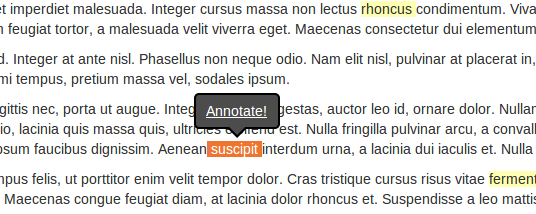
\includegraphics[height=3.2cm]{../PIC/annotate}\quad
  %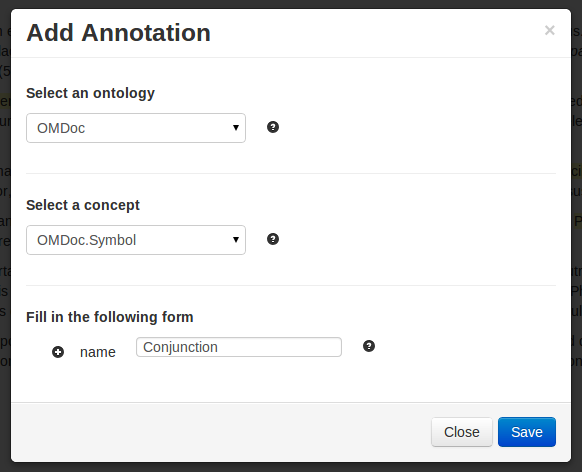
\includegraphics[height=3.1cm]{../PIC/add-symbol}
  \caption{Annotating in KAT: Selection and Form-Filling}\label{fig:kat-annotate}
\end{figure}
